
\begin{figure*}
	\center
	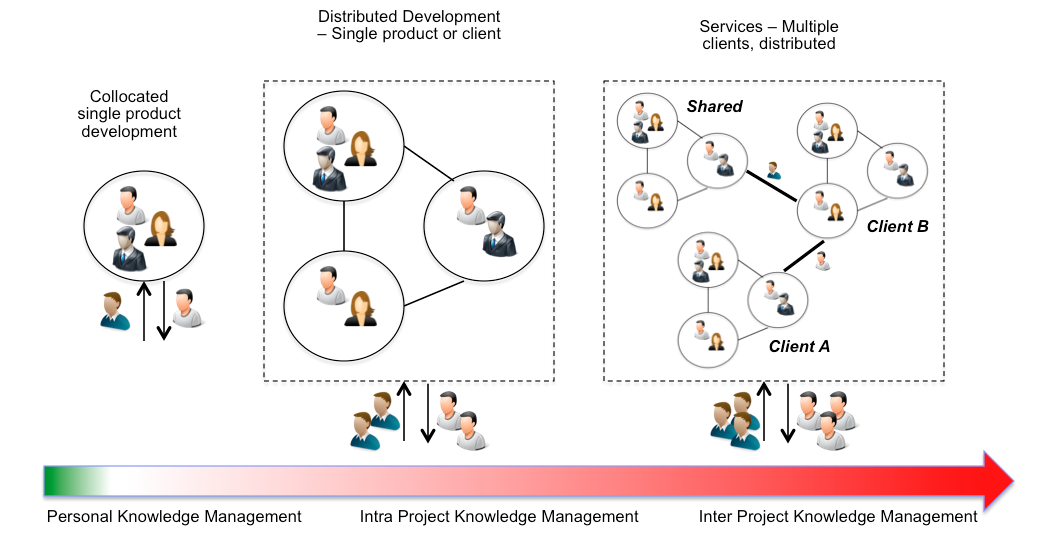
\includegraphics[scale=0.7]{figs/km-types.png}
	\caption{Team structures and knowledge management needs}
	\label{fig-km}
\end{figure*}

\begin{figure*}
	\center
	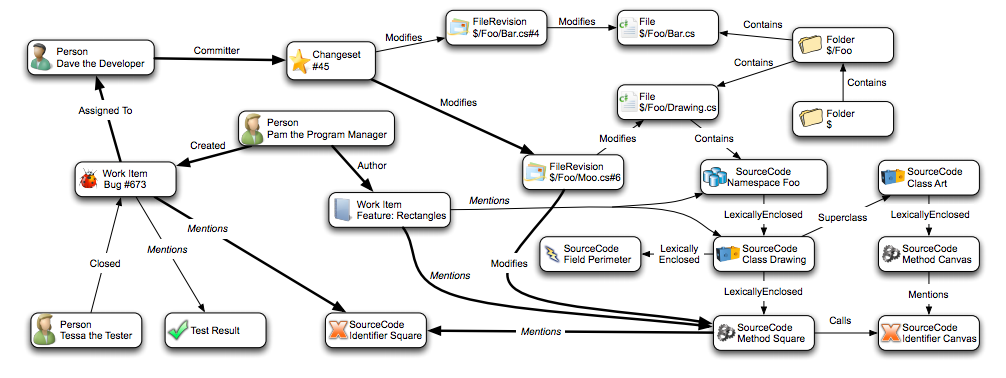
\includegraphics[scale=0.4]{figs/codebook.png}
	\caption{Project Network Example from Codebook}
	\label{fig-codebook}
\end{figure*}

\section{Knowledge Management}
\label{sec:km}

Software development is inherently a knowledge intensive activity. Software designers and developers leverage their software development skills along with knowledge about the domain, past experiences and knowledge of team members, to solve the current problem at hand, be it implementing a new feature/application or solving a bug. 
In small, colocated teams, knowledge management is not a big challenge. Who is an expert on what part of the system is typically known. New team members coming in would use informal channels of communication to figure out who are the experts on the system. If need be, individuals can tap into the knowledge of these experts to quickly address task at hand. 

Knowledge management starts to become a challenge when team size increases and/or teams start getting distributed geographically. In large teams or distributed environments, the requisite knowledge of the system---expertise, dependencies, best practices and so on---is spread across multiple people, locations and even organizations (in cases such as outsourcing) \cite{Desouza:2006}. In such projects, a knowledge management system is needed to create so called project memories that primarily help with following needs. Firstly, they enable new joinees to understand the project with little face to face guidance. Help them identify experts in the project who they can reach out to in case they have queries. Secondly, they enable existing team members to identify artifacts relevant for their current task and people they might need to coordinate with. 

Now consider the case for services organizations such as IBM that are in the business of developing and managing software systems for multiple clients. Day in and day out different employees are churning out new features, resolving issues, implementing new applications for different clients. While each client is different, there is ample scope of reusing best practices and even solutions from past engagements to achieve greater efficiency and efficacy in present and future projects. Consider the following example, for \textit{client A} there is a need to implement a payroll system. Before starting the project, it would be beneficial to know if a similar system was implemented for some other client, what were the design considerations and challenges faced and if the complete solution could be reused in whole or parts. As another example consider the following scenario, \textit{developer Foo} has been asked to fix an issue related to leave planning on an application implemented using \textit{SAP's Human Capital Management (HCM)} module. It so happens that \textit{HCM} implementation has been done for multiple clients by the organization. It could potentially help \textit{Foo} if he were to know if similar issue was reported in any other implementations and how it was resolved. Hence, at an organization level there is again a need for a knowledge management solution to can act as organization memory \cite{Stein:1995} that helps quickly identify if a similar task (where a task could be a bug to be resolved, an application to be developed or a project risk that needs to be addressed) has been done for another client and if yes, what parts of solution could be reused.

As illustrated in figure~\ref{fig-km}, services organizations need to manage knowledge at all three levels: personal, project and organization. It is believed that individuals are adept at managing their own knowledge and drawing upon it when a new situation comes in \cite{Bruce:2005}. For example, a developer who has been assigned a bug on a system (s)he has implemented would typically know where to start investigation from because of prior knowledge about the system. A project manager working long enough in the product would know the primary risks associated with the project, fault prone areas and so on. However, system support is needed (in form of tools and processes) to effectively manage knowledge at project and organization level primarily because of number of people involved, diversity in their experience and skill levels, geographical distribution and large amount of resource churn.  

\subsection{Examples of Knowledge Management Solutions}

What kind of knowledge management systems do services organizations use today? What are the capabilities these systems offer and what challenges do they address? In this section we attempt to answer these questions by presenting existing instances of project knowledge management system and organization knowledge management systems. 

\subsubsection{Project Knowledge Management Systems} 

In context of distributed development projects such as Hipikat\cite{} and Codebook\cite{} have attempted to create knowledge management systems that can serve as project memories. The basic premise in both these systems is that people involved in the project should not be spending extra time authoring data for the knowledge base. Artifacts and other information being produced as part of SDLC should be enough to populate the database and derive useful information. Existing artifacts in the project such as code, requirements, bugs, communication serve as data in the repository. Artifacts are linked to each other via available traceability information e.g. a bug is linked to code files that we modified to fix it or communication that happened around the bug. Artifact to people relationships are created based on who created and/or modified an artifact. The project database is essentially a network of artifacts and people, an example is shown in Figure~\ref{fig-codebook}. The knowledge management system then provides capabilities to search based on textual content of the artifacts and further do regular language reachability queries on the network. The usage of these systems will become clear from following examples.\\
\\
{\bf Example from Hipikat}\\
\\
\textit{Scenario}: How will a software developer use information from the project memory about past modifications completed on the project to help them in a current modification task? \\\textit{Usage}: Given the modification request, developer identifies a set of keywords (s)he that summarize the issue he is handling and uses it to query the project database. If it's a bug report, developer can use the complete bug report to search the system. The system uses textual search to identify previous tasks similar to one the developer is working on now. Additionally it also suggests arifacts and people that are transitively linked to these textually similar results. A bug report returned in search result is linked to code files modified to fix the bug and developer who resolved the bug in past. The developer can flip through the search results to see if anything of interest comes up and use that information to solve current issue at hand.\\
\\
{\bf Example from Codebook}\\
\\ 
\textit{Scenario}: How will a bug triager use project memory to assign the bug to correct software developer? \\
\textit{Usage}: Given the bug, the triager does some initial investigation to identify what is the fault causing module. Once the module is identified (s)he identifies the owner of the module by checking on who has made the most number of changes to that module (code->change history-> people linkage) or who has fixed most bugs for that module and assigns the bug to that person.
\\
\\
As is evident from above examples, the richness of the artifact to artifact to people graph determines how much knowledge is there in the system. So the biggest challenge here is getting complete end to end traceability between different formal artifacts and informal artifacts being produced during SDLC into the system. If different tools are used to author different artifacts such as using Microsoft Word to author requirements, CVS to maintain code and using emails to do discussions, then traceability creation and maintanence becomes a chore. However, in the recent years there has been increasing use of complete Application Lifecycle Management solutions such as \textit{Rational Team Concert}, \textit{SAP Solution Workbench}, \textit{Mylyn integrated CVS/SVN/Git/Jira}, that allow a project to manage all stages of the project---requirements, design, code, testing, task management---from a single tool. These ALM solutions make it easier for people to specify relationship between different artifacts as they are doing the work. E.g. a developer is assigned a work item in RTC, (s)he does discussion with project manager and architect on the work item from within the tool itself and then makes some code changes and attaches the change set to the work item.  When an ALM solution is getting used, then creating the project network is a matter of crawling the data from the ALM system. There have also been works that try to infer relationships between artifacts using potentially referential information\cite{}. For example, if making a code commit, the developer puts in a comment like \textit{Fixed Bug \#145}, then with high confidence the change is to fix \textit{Bug \#145} and corresponding edge between code file and bug report can be created. For retrieving information, the KMS provides search capabilities primarily based on textual similarity between query and content and ability to navigate through edges in the graph to derive additional insights. 

\subsubsection{Organization Knowledge Management System}

The goal behind organization knowledge management is to ensure that knowledge available with any of it's past or current employees can be made available to another employee when the need arises. How to effectively share knowledge within an organization is a much studied management discipline \cite{}. Two strategies for knowledge management are typically employed, codification or personalization \cite{}. In codification knowledge is carefully captured and stored in the database, where it can be accessed and used by anyone in the company. In this approach, the information is extracted from the person who developed it, made independant of that person, and reused for various purposes. After removing all client-sensitive information, all data related to a solution, decision or incident is collated, put in a database and made available for everyone to use. This strategy allows many people to search for and retrieve codified knowledge without having to contact the person who originally developed it. This opens up the possibility of achieving required scale in knowledge reuse in services organizations and is also able to handle the high amount of resource churn. Further, this strategy is effective where knowledge to be shared is explicit such as software code, market data. In personalization,knowledge is typically tied to person who developed is and is shared mainly through direct person-to-person contacts. The chief purpose of knowledge management system here is to help people find and connect to other people who have requisite knowledge, not to store it. This strategy works well in cases where the knowledge to be shared is tacit such as project judgements under risk, technology/business expertise, and cannot be used as it. Personal contact is needed to communicate the background, thinking and past decision made and brainstorming is needed to apply learning in a new situation. Though it is difficult to achieve high scale with this strategy, if enough experts are available in an organization, then this strategy is helpful for sharing knowledge that is difficult to codify. 

Now we present two knowledge management system in use within IBM that attempt to promote knowledge reuse across projects, albeit for different purposes. The first one refered to as Wisdom\cite{} is a knowledge base of problem tickets resolved across various clients where IBM is responsible for application maintanence. The other one refered to as Consultant Assistant\cite{} is a knowledge base to promote software reuse. \\
\\
{\bf Reuse of information in Problem Tickets using Wisdom}\\ 
\\
In large software service providers like IBM, Accenture software being developed for different clients might not all be custom. In many cases, packaged applications such as \textit{SAP} and \textit{Oracle} and/or COTS products are getting used and client specific customizations done on top of them. When a client faces an issue with some application of their's they open a problem ticket. The cause of the problem ticket could be the customization done for client or some issue with the way COTS was used or some bug in COTS itself. If the issue is with the configuration or with COTS itself, then it is highly likely that same issue has been resolved in context of some other client earlier too. With Wisdom IBM created a cross-account repository of all past problem tickets resolved. Each ticket has information description of problem and how it was resolved. This is the typical information captured in the ticket as it goes through the resolution process. Before putting the ticket in a shared repository, it is cleansed of any client specific private information such as people names, phone numbers etc. Along with every ticket, additional information is saved about client landscape i.e. whether the issue was on \textit{SAP HCM} or \textit{Websphere Application Server} or so on. When anyone within IBM is assigned a problem ticket, they can search through the repository to see if similar issue was resolved in the past. Because of large number of accounts being serviced by IBM, the repository quickly grew to a size of 750K tickets in a small period of time. It was a conscious decision to not do any manual curation of information, as past experiences with KMS have shown that when people have to specifically harvest information from their existing work then KMS is likely to get out of date soon because of extra motivation required to author content, cost cutting etc \cite{}. 

However, because of this decision quite a few useless tickets i.e. tickets that did not have proper resolution data were getting into the system. If people do not find relevant solution in top couple of search results then they develop a perception that system is not useful and do not end up coming back. To handle this situation, the KMS was enhanced to provide a quality score to each ticket coming in the system. This quality metric was calculated using the amount of technical useful content in the ticket versus non-technical content \cite{}. During search, besides textual similarity, ticket quality and recency were used as additional measures to determine the ranking of a ticket in the search results. 

The second challenge that we faced in promoting usage was the amount of information a user might potentially need to go through before identifying whether the returned problem tickets are applicable to his/her problem or not. Problem tickets might vary from a couple of lines to thousands. Hence, automatic summarization of bug reports~\cite{} was another feature that was needed in the system to reduce the amount of data a user might need to go through. Further, multiple tickets might be talking of same problem and followed same resolution. So it was necessary that content duplicates in search results were detected and grouped together. Detecting duplicate bug reports is a well studied area \cite{} and was applicable here. Another issue with retrieval was that while problem symptom might be the same, the root cause might be different. So, clustering of problem tickets was needed to highlight these different topics under tickets that seem similar. 

Finally, in cases where the users did not find the codified information enough, a need was felt to follow a socialization approach i.e. connect them to other people in the organization who might have solved similar issues, specifically highlighting those that are in the same project and/or location and/or already belong to their social network. Figure ~\ref{fig:wisdom} shows a snapshot from the Wisdom system.\\
\\
{\bf Software Reuse using Consultant Assistant}\\
\\


\subsection{Research Directions}
